O método da paralaxe consiste, basicamente, em observar um objeto a partir de dois pontos de vista diferentes.

Paralaxe é, justamente, o deslocamento aparente observado na direção do objeto devido à mudança de posição do observador.

\begin{figure}[!htb]
    \centering
    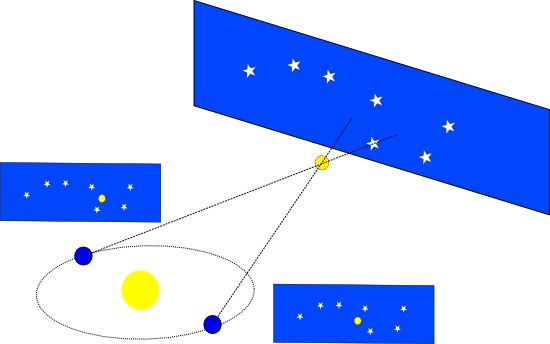
\includegraphics[scale=0.4]{capítulos/cap1/imagens/ParallaxeV2.png}
    \caption{Fonte: Wikipedia}
    \label{fig:my_label}
\end{figure}

Agora podemos encontrar uma expressão, baseando-se na Paralaxe, para encontrar distância.

\begin{figure}[!htb]
   \centering
   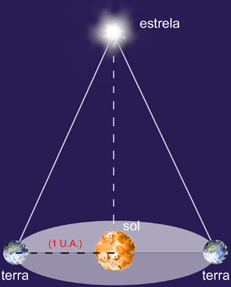
\includegraphics[scale=0.6]{capítulos/cap1/imagens/solfundoclaro.jpg}
\end{figure}
\newpage
É possível notar triângulos retângulos na imagem, então podemos associar uma função trigonométrica.

$$tan \ \alpha = \frac{1 A.U}{d} \Rightarrow d = \frac{1 A.U}{tan \ \alpha} $$

Onde \textit{d} é a distância do Sol à estrela. Sabe-se que $tan \ \alpha = \frac{sen \ \alpha}{cos \ \alpha}$ e expandindo o seno e o cosseno em séries de Taylor até segunda ordem (fazemos até n=2. Os outros termos são pequenos, são considerados termos de correção e fazem pouca diferença em pequenos ângulos então "podem" ser ignorados, mania de físico) temos:

$$f(x) = \sum_{n=0}^{\infty} \frac{f^{n}(a)}{n!}(x-a)^n$$

Essa é a série de Taylor de $f(x)$ centrada em $x=a$.

Para o seno, temos:

$$f(x) = sen(x) \Rightarrow f(0) = 0 \ ,  f'(0) = 1 \ , f"(0) = 0$$

Para o cosseno, temos:

$$f(x) = cos(x) \Rightarrow f(0) = 1 \ ,  f'(0) = 0 \ , f"(0) = -1$$

Então, fazendo nossa aproximação, chegamos em \footnote{Outro jeito seria considerar o famoso caso de "pequenas oscilações".}:

$$sen(\alpha) \approx \alpha , \ cos(\alpha) \approx 1 \Rightarrow tan(\alpha) \approx \alpha$$


Ora, já que $tan(\alpha) \approx \alpha$ então\footnote{É possível também fazer essa dedução considerando \textit{d} a distância entre a Terra e o alvo.}:

\begin{equation}
    d = \frac{1}{\alpha}
    \label{distância}
\end{equation}

A unidade de medida da distância é o \textbf{parsec} (paralaxe + second of arc).



